\section{Theorie}
\label{sec:Theorie}

In diesem Versuch wird die Beugung des Lichtes am Einzel- und Doppelspalt untersucht. Hierbei ist der
Wellencharakter des Lichtes von besonderer Bedeutung. Mit Hilfe der Beugungsbilder sollen Rückschlüsse 
auf die Geometrie der Spate geschlossen werden. 

Lichtbeugung tritt dann auf, wenn die Größe der verursachenden Hindernisse in der Größenordnung der 
Wellenlänge $\lambda$ des Lichtes liegt. Es gibt zwei grundlegende Versuchsanordnung, um diese Beugung
zu untersuchen: Die Anordnung nach Frauenhofer und die nach Fresnel. Beide sind in Abbildung \ref{fig:Beugungen} 
dargestellt.

\begin{figure}
  \centering
  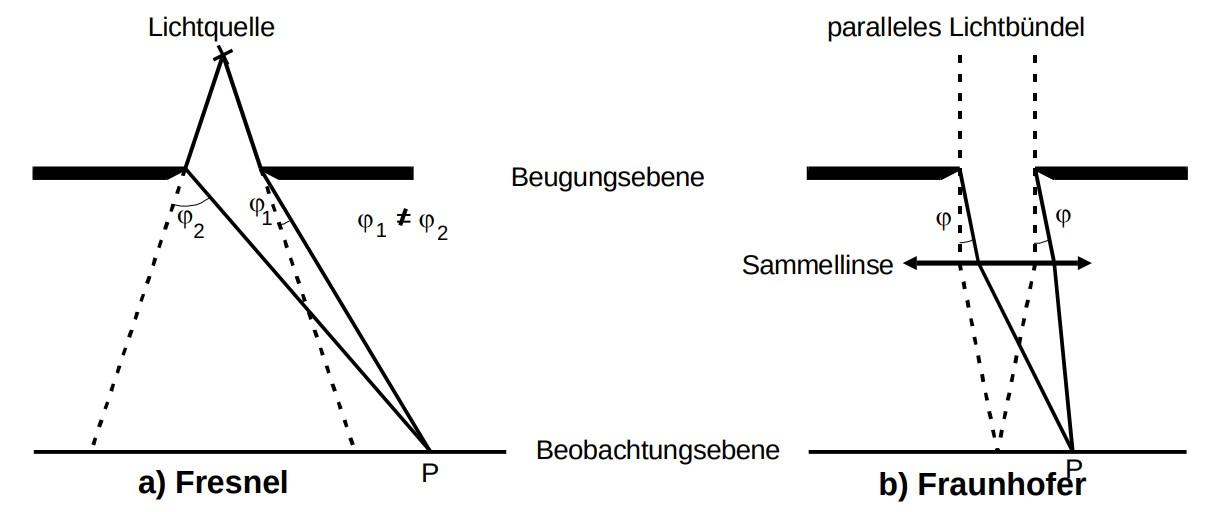
\includegraphics[scale=0.3]{content/Begungen.jpg}
  \caption{Freschnelsche und Frauenhofer Beugung an einem Spalt.[1]}
  \label{fig:Beugungen}
\end{figure}

Bei dem Aufbau nach Fresnel liegen sowohl die Bildebene als auch die Punktquelle im Endlichen. Dies 
führt dazu, dass die Lichtstrahlen unter verschiedenen Winkeln im Interferenzpunkt einfallen. Unter einer
Verschiebung der Lichtquelle ins Unendliche resultiert stattdessen ein paralleles Lichtbündel mit einer 
ebenen Wellenfront. Dadurch interferieren im Punkt $P$ nur diejenigen Lichtstrahlen, die unter dem gleichem 
Winkel $\Phi$ gebeugt werden. \\
Dies entspricht der Betrachtung von Frauenhofer. Diese Nährung ist mathematisch 
relativ einfach zu beschreiben, weswegen in diesem Versuch nur diese betrachtet wird.\\ 

In diesem Versuch werden sowohl die Beugungseffekte an einem Einfachspalt als auch an einem 
Doppelspalt betrachtet. 

\subsection{Einfachspalt}

Als Untersuchungsobjekt wird ein Spalt angenommen, dessen Länge sehr groß gegen die Breite sei, sodass 
das Lichtbündel nur in einer Koordinate begrentzt wird. Wenn nun eine ebene Welle (realisiert durch Linsen)
auf diesen Spalt trifft, findet das Huygensche Prinzip Anwendung. Dies besagt, dass 
von jedem beliebigen Punkt einer Wellenfront eine Kugelwelle ausgeht. Durch Überlagerung dieser Kugelwellen
ergibt sich eine neue Wellenfront, die die Einhüllende der ausgesandten Kugelwellen ist. \\
Um den Zustand 
an einem Punkt der Wellenfront zu beschreiben, gelingt dies durch eine Überlagerung aller Kugelwellen, die
zu einem bestimmten Zeitpunkt dort ankommen. Es ist also nötig über alle Strahlenbündel zu summieren, die 
unter einem Winkel $\Phi$ abgelenkt werden, um die Amplitude zu bestimmen. Dieses Strahlenbündel ist klein, 
sodass diese Integration in eine über die Spaltbreite $b$ übergeht. 
Die einfallende Welle wird durch 

\begin{equation*}
A(z,t) = A_0\exp{\left(i(\omega t - 2\pi\frac{z}{\lambda})\right)}
\end{equation*}

beschrieben. Die Phasendifferenz von zwei Strahlen die in der Strahlebene den Abstand $x$ besitzen, wie 
in Abbildung \ref{fig:Phase} dargestellt, beträgt nun 

\begin{equation*}
\delta = \frac{2\pi x\sin{(\Phi)}}{\lambda}. 
\end{equation*}

\begin{figure}
  \centering
  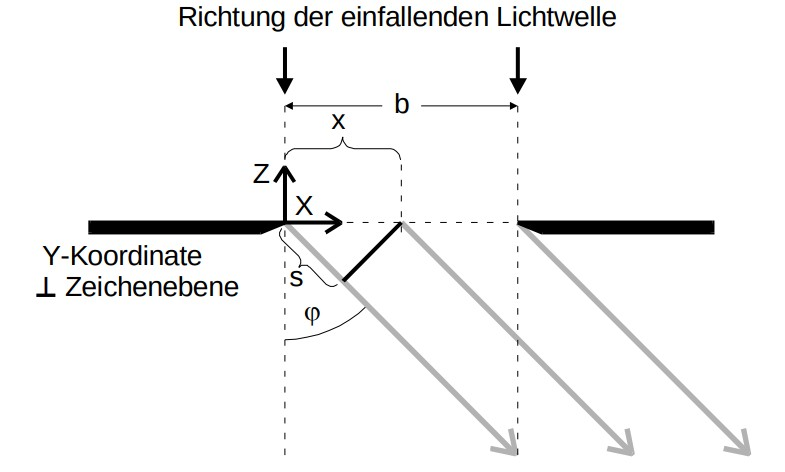
\includegraphics[scale=0.3]{content/Phase.jpg}
  \caption{Skizze zur Ableitung einer Phasenbeziehung zwischen 2 Teilstrahlen bei der Fraunhoferschen
Beugung am Spalt. [1]}
  \label{fig:Phase}
\end{figure}

Nach Ausführung der Integration und einigen Umformung ergibt sich schließlich für die Amplitude 
des in $\Phi$-Richtung abgelenkten Strahlenbündels: 

\begin{equation*}
B(z,t,\phi) = A_0 \exp{\left(i\left(\omega t - \frac{2\pi z}{\lambda}\right)\right)}\cdot \exp{\left(\frac{\pi i b \sin{(\Phi)}}{\lambda}\right)}\cdot
\frac{\lambda}{\pi \sin{(\Phi)}}\sin{\left(\frac{\pi b \sin{(\Phi)}}{\lambda}\right)}.
\end{equation*}

Die beiden Exponentialfunktionen stellen dabei nur Phasenfunktionen dar, wobei die Erste die Orts- und Zeitabhängigkeit 
der Amplitude beschreibt und die Zweite einen richtungsabhängigen Phasenvektor darstellt. Daraus ergibt sich, dass nur 
die letzten beiden Terme für experimentelle Untersuchungen relevant sind. Da sich die Amplitude nicht direkt 
messen lässt wird nun die zeitlich gemittelte Intensität betrachtet. Dabei gilt: 

\begin{equation}
I(\Phi) \propto B(\Phi)² = A_0² b² \left(\frac{\lambda}{\pi b \sin{(\Phi)}}\right)²\cdot \sin²{\left(\frac{\pi b \sin{(\Phi)}}{\lambda}\right)}.
\label{eqn:einfach}
\end{equation}

Diese wird niemals negativ und besitzt bei den Nulldurchgängen der Amplitudenfunktion $B(\Phi)$ Minima. 

\subsection{Doppelspalt}

Die mathematische Betrachtung erfolgt analog zu der des Einzelspalts. Er wird als Überlagerung zweier Einzelspalte
der Breite $b$ betrachtet, die sich im Abstand $s$ zueinander befinden. Dann ergibt sich die Intensitätsverteilung
zu: 

\begin{equation}
I(\Phi) \propto B(\Phi)² = A_0 \cos²{\left(\frac{\pi s \sin{(\Phi)}}{\lambda}\right)}\cdot \left(\frac{\lambda}{\pi b \sin{(\Phi)}}\right)² 
\cdot \sin²{\left(\frac{\pi b \sin{(\Phi)}}{\lambda}\right)}. 
\label{eqn:doppel}
\end{equation}

Diese Verteilung entspricht der des Einzelspaltes multipliziert mit einem $cos²$-Term. Dies führt zu zusätzlichen
Minima. 

\subsection{Fourier-Transformation}

Die Amplitudenverteilung der Frauenhofer Beugung ist auch allgemeiner zugänglich, denn es zeigt sich, 
dass $B(\Phi)$ als Fouriertransformierte der Amplitudenverteilung der einfallenden Welle in der 
Beugungsebene aufgefasst werden kann. Wird $f(x)$ durch 

\begin{equation*}
\int_{-\infty}^{\infty} f(x) \exp{\left(ix\gamma\right)}
\end{equation*}

in ihre Fouriertransformierte $g(\gamma)$ transformiert, so lässt sich diese durch geschickte Wahl von 
$\gamma$ mit der Amplitudenverteilung, bisher als $B(\Phi)$ bezeichnet, identifizieren. Im Vorliegendem 
Fall des Einzelspaltes sei $f(x)$ gegeben als:

\begin{equation*}
f(x) = 
\begin{cases}
A_0, & 0 \le x \le b\\
0  , & \text{sonst} 
\end{cases}
\end{equation*}

Wird dies in $g(\gamma)$ eingesetzt und daraufhin die Eulersche Formel angewendet, so ergeben sich Übereinstimmungen
von $g(\gamma)$ und $B(\Phi)$ mit 

\begin{align*}
\gamma &= \frac{2\pi\sin{(\Phi)}}{\lambda},\\
g(\gamma) &= \frac{2 A_0}{\gamma} \cdot \exp{\left(\frac{i\gamma b}{2}\right)}\cdot \sin{\left(\frac{\gamma b}{2}\right)}.
\end{align*}

Hieraus ergibt sich, dass die Fouriertransformierte das Huygensche Prinzip mathematisch formuliert. 

